\section{Описание}
Для корректной работы моделей признаки нужно нормализовать. Сначала разделим данные на тренировучную и тестовую выборку, после чего нормализуем их.
Делаем это именно в таком порядке, чтобы у нас было гарантировано, что и в тренировочной, и в тестовой выборке все значения будут от 0 до 1.
Данные разделим в пропоциях (80 к 20), используя используя train\_test\_split из scikit-learn \cite{scikit-split}.
scikit-learn позволяет сделать это с помощью normalize \cite{scikit-normalize}, я использую метрику <<max>>.


В задании требуется сделать все модели совместимыми с scikit-learn \cite{scikit-develop}, поэтому получение оценок модели \cite{ml-metrics} 
можно сделать методами из этой же библотеки:
\begin{lstlisting}[language=Python]
def scores(model, X, y_true):
    y_pred = model.predict(X)
    print("Accuracy:", accuracy_score(y_true, y_pred))
    print("Recall:", recall_score(y_true, y_pred))
    print("Precision:", precision_score(y_true, y_pred))
    figure = plt.figure(figsize = (20, 5))
    matr = confusion_matrix(y_true, y_pred)
    ax = plt.subplot(1, 2, 1)
    ConfusionMatrixDisplay(matr).plot(ax = ax)
    ax = plt.subplot(1, 2, 2)
    RocCurveDisplay.from_predictions(y_true = y_true, y_pred = y_pred, name = "ROC-curve", ax = ax)
    plt.show()
\end{lstlisting}

При реализации моделей я использовал шаблон \cite{scikit-github} из scikit-learn, в котором учтены все тонкости реализации: наследование 
от нужных классов (ClassifierMixin, BaseEstimator) и необходимые методы (fit, predict).
\pagebreak

\subsection{Метод k-ближайших соседей}
Среди всех объектов обучающей выборки ищем k ближайших, среди них классифицируем объект тем классом, которого больше всего среди соседей:
\begin{lstlisting}[language=Python]
class kNN(BaseEstimator, ClassifierMixin):
    
    def __init__(self, k=1):
        self.k = k

    def fit(self, X, y):
        X, y = check_X_y(X, y)
        # Store the classes seen during fit
        self.classes_ = unique_labels(y)

        self.X_ = X
        self.y_ = y
        self.is_fitted_ = True
        # `fit` should always return `self`
        return self

    def predict(self, X):
        # Check is fit had been called
        check_is_fitted(self, ['X_', 'y_'])

        # Input validation
        X = check_array(X)

        y = np.ndarray((X.shape[0],))
        for (i, elem) in enumerate(X):
            distances = euclidean_distances([elem], self.X_)[0]
            indexes = np.argsort(distances, kind='heapsort')[:self.k]

            labels, cnts = np.unique(self.y_[indexes], return_counts=True)
            y[i] = labels[cnts.argmax()]
        return y
\end{lstlisting}
Использую Евклидову метрику из scikit-learn для вычисления расстояний и метод argpsort из numpy \cite{numpy-argsort} для индексной сортировки.
Также в качестве алгоритма сортировки использую heapsort, т.к. по умолчанию используется quicksort, который, исходя из документации, имеет 
оценку сложности $O(n^2)$, в то время как heapsort сортирует массив за $O(n \cdot log(n))$, при этом не используя дополнительную память 
(исходя из документации numpy)
\begin{center}
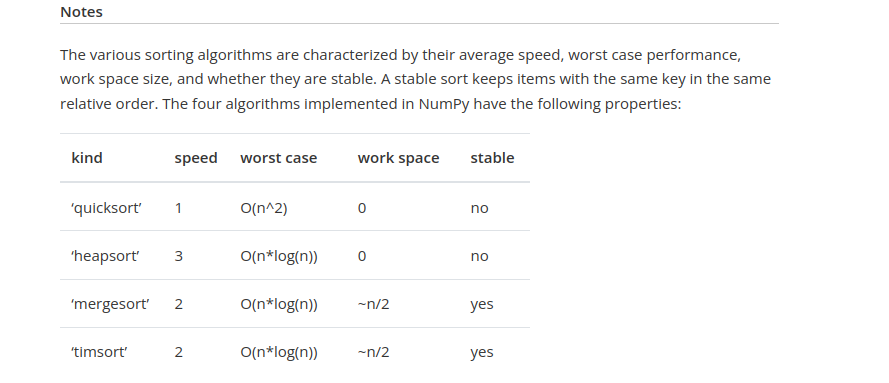
\includegraphics[scale=0.65]{./images/doc}
\end{center}
Из отсортированных индексов получаю k ближайших соседей.
\pagebreak

\subsection{Логистическая регрессия}
Логистическая регрессия по сути является однослойной нейросетью. Использую результаты из ЛР по реализации собственного фреймворка, чтобы 
реализовать модель. Описываю класс сети, которую можно строить из разных слоёв:
\begin{lstlisting}[language=Python]
import matplotlib.pyplot as plt
class Net:
    def __init__(self, loss_function=CrossEntropyLoss()):
        self.layers = []
        self.loss_func = loss_function

# ----Net's standart methods----
    def add(self,l):
        self.layers.append(l)

    def forward(self,x):
        for l in self.layers:
            x = l.forward(x)
        return x

    def backward(self,z):
        for l in self.layers[::-1]:
            z = l.backward(z)
        return z

    def update(self,lr):
        for l in self.layers:
            if 'update' in l.__dir__():
                l.update(lr)
# ----end Net's standart methods----

# ----loss functions----
    def forward_loss(self, x, y):
        p = self.forward(x)
        return self.loss_func.forward(p, y)

    def backward_loss(self, l):
        dp = self.loss_func.backward(l)
        return self.backward(dp)

    def _update_dry(self, x, y, step):
        self.update(step)
        loss = self.forward_loss(x, y)
        self.update(-step)
        return loss
# ----end loss functions----

# ----Net train----
    def _is_less_update_dry(self, x_dry, y_dry, step, l_dry, r_dry):
        lhs = (2.0 * l_dry + r_dry) / 3.0
        rhs = (l_dry + 2.0 * r_dry) / 3.0

        loss_lhs = self._update_dry(x_dry, y_dry, step * lhs)
        loss_rhs = self._update_dry(x_dry, y_dry, step * rhs)

        return loss_lhs < loss_rhs

    def train_epoch(self, epoch_train_x, train_labels, batch_size=100, step = 1e-7):
        for index in range(0, len(epoch_train_x), batch_size):
            xb = epoch_train_x[index:index + batch_size]
            yb = train_labels[index:index + batch_size]

            loss = self.forward_loss(xb, yb)
            self.backward_loss(loss)

            l = 1.0
            r = 5e2
            while r - l < 0.01:
                lhs = (2.0 * l + r) / 3.0
                rhs = (l + 2.0 * r) / 3.0
                if self._is_less_update_dry(xb,yb,step, lhs, rhs):
                    r = rhs
                else:
                    l = lhs
            self.update(r * step)
\end{lstlisting}
\pagebreak

Линейный слой сети с возможностью обновления весов (изначально матрица весов заполняется случайными числами, а вектор смещения нулями) так же вынесен в отдельный класс:
\begin{lstlisting}[language=Python]
class Linear(Layer):
    def __init__(self, nin, nout):
        sigma = 1.0 / np.sqrt(2.0 * nin)
        self.W = np.random.normal(0, sigma, (nout, nin))
        self.b = np.zeros((1, nout))
        self.dW = np.zeros_like(self.W)
        self.db = np.zeros_like(self.b)

    def forward(self, x):
        self.x = x
        return np.dot(x, self.W.T) + self.b

    def backward(self, dz):
        dx = np.dot(dz, self.W)
        dW = np.dot(dz.T, self.x)
        db = dz.sum(axis=0)
        self.dW = dW
        self.db = db
        return dx

    def update(self, lr):
        self.W -= lr * self.dW
        self.b -= lr * self.db
\end{lstlisting}
В логистической регрессии используется функция активации сигмоида, которая так же описана в отдельном классе:
$$\sigma(x) = (1 + e ^ {-x}) ^ {-1}$$
\begin{lstlisting}[language=Python]
class Sigmoid(Layer):
    def forward(self, x):
        self.y = 1.0 / (1.0 + np.exp(-x))
        return self.y

    def backward(self, dy):
        return self.y * (1.0 - self.y) * dy
\end{lstlisting}
\pagebreak

В качестве функции потерь использую binary cross entropy loss, так как стоит задача бинарной классификации:
\begin{lstlisting}[language=Python]
class BinaryCrossEntropy(Layer):
    def forward(self, p, y):
        y = y.reshape((y.shape[0], 1))
        self.p = p
        self.y = y
        res = y * np.log(p) + (1 - y) * np.log(1 - p)
        return -np.mean(res)

    def backward(self, loss):
        res = (self.p - self.y) / (self.p * (1 - self.p))
        return res / self.p.shape[0]
\end{lstlisting}
Логистическая регрессия содержит нейросеть, состояющую из линейного слоя, сигмиоды и описанной выше функции потерь. Также есть настраиваемый 
параметр, который характеризует кол-во входных признаков.
Алгоритм обучения сети --- стохастический градиентный спуск с постоянным шагом:
\begin{lstlisting}[language=Python]
class LogisticRegression(ClassifierMixin, BaseEstimator):
    def __init__(self, epoches=1, batch_size=10, SGD_step=0.001, nin=10):
        self.epoches = epoches
        self.batch_size = batch_size
        self.SGD_step = SGD_step
        self.nin = nin
        self.Net = Net(BinaryCrossEntropy())
        self.Net.add(Linear(nin, 1))
        self.Net.add(Sigmoid())

    def fit(self, X, y):
        # Check that X and y have correct shape
        X, y = check_X_y(X, y)
        # Store the classes seen during fit
        self.classes_ = unique_labels(y)

        self.X_ = X
        self.y_ = y
        for _ in range(self.epoches):
            self.Net.train_epoch(X, y, self.batch_size, self.SGD_step)
        # Return the classifier
        return self

    def predict(self, X):
        # Check is fit had been called
        check_is_fitted(self, ['X_', 'y_'])

        # Input validation
        X = check_array(X)

        y = self.Net.forward(X)
        res = np.where(y < 0.5, 0, 1)
        return res

    def getW(self):
        return self.Net.layers[0].W

    def getb(self):
        return self.Net.layers[0].b
\end{lstlisting}
\pagebreak

\subsection{Метод опорных векторов}
Метод похож на предыдущий, но функция ошибки требует сами данные, на которых происходит обучение, поэтому встроить в класс сети не получилось.
Однако, из-за схожести архитектуры реализации было принято решение создать класс, который наследуется от Net, написанного в ЛР по персептронам.
На основе этого класса отдельно описываю модель опорных векторов с мягким зазором:
\begin{lstlisting}[language=Python]
class SoftMarginSVM(Net):
    def __init__(self, nin, alpha):
        super().__init__()
        self.alpha = alpha
        sigma = 1.0 / np.sqrt(nin)
        self.W = np.random.normal(0., sigma, (1, nin + 1))

    def forward(self, x):
        z = np.dot(x, self.W.T)
        return z

    def add_ones(self, x):
        ones = np.ones((x.shape[0], 1))
        return np.hstack((x, ones))

    def predict(self, x):
        res = self.forward(self.add_ones(x))
        return np.where(res < 0, 0, 1)

    def train_epoch(self, x, y, batch_size=100, step=1e-7):
        x = self.add_ones(x)
        y = np.where(y > 0, 1, -1)
        for i in range(0, len(x), batch_size):
            xb = x[i:i + batch_size]
            yb = y[i:i + batch_size]

            pred = self.forward(xb)
            grad = self.alpha * self.W
            for i in range(len(xb)):
                if (yb[i] * pred[i] < 1):
                    grad -= yb[i] * xb[i]
            self.W -= step * grad
\end{lstlisting}
Класс получился простой, но не очень универсальный. Чтобы отбросить вектор смещения $b$, я ввёл искуственный признак, 
который всегда равен единице \cite{habr-svm}.
\pagebreak

Эта модель затем встраивается в классификатор. Параметры почти такие же, как и в случае с логистической регрессией:
\begin{lstlisting}[language=Python]
class SVM(ClassifierMixin, BaseEstimator):
    def __init__(self, epoches=1, batch_size=10, SGD_step=0.001, alpha=0.1, nin=10):
        self.epoches = epoches
        self.batch_size = batch_size
        self.SGD_step = SGD_step
        self.nin = nin
        self.alpha = alpha
        self.Net = SoftMarginSVM(nin, alpha)

    def fit(self, X, y):
        # Check that X and y have correct shape
        X, y = check_X_y(X, y)
        # Store the classes seen during fit
        self.classes_ = unique_labels(y)

        self.X_ = X
        self.y_ = y
        for _ in range(self.epoches):
            self.Net.train_epoch(X, y, self.batch_size, self.SGD_step)
        # Return the classifier
        return self

    def predict(self, X):
        y = self.Net.predict(X)
        return y

    def getW(self):
        return self.Net.W
\end{lstlisting}
\pagebreak

\subsection{Наивный байесовский классификатор}
Идея модели в наивном предположении о независимости параметров. Так же часто используется модель с нормальным распределением признаков.
\begin{lstlisting}[language=Python]
class NaiveBayes(ClassifierMixin, BaseEstimator):
    def __init__(self):
        None

    def fit(self, X, y):
        # Check that X and y have correct shape
        X, y = check_X_y(X, y)

        self.X_ = X
        self.y_ = y

        labels, cnts = np.unique(self.y_, return_counts = True)
        self.labels = labels
        self.p_of_y = np.array([elem / self.y_.shape[0] for elem in cnts])
        self.means = np.array([self.X_[self.y_ == elem].mean(axis = 0) for elem in labels])
        self.stds = np.array([self.X_[self.y_ == elem].std(axis = 0) for elem in labels])
        # Return the classifier
        return self

    def gaussian(self, mu, sigma, x0):
        return np.exp(-(x0 - mu) ** 2 / (2 * sigma)) / np.sqrt(2.0 * pi * sigma)

    def predict(self, X):
        # Check is fit had been called
        check_is_fitted(self, ['X_', 'y_'])

        # Input validation
        X = check_array(X)

        res = np.zeros(X.shape[0])
        for (i, elem) in enumerate(X):
            p = np.array(self.p_of_y)
            for (j, label) in enumerate(self.labels):
                p_x_cond_y = np.array([self.gaussian(self.means[j][k], self.stds[j][k], elem[k]) for k in range(X.shape[1])])
                p[j] *= np.prod(p_x_cond_y)
            res[i] = np.argmax(p)
        return res
\end{lstlisting}
\pagebreak

\subsection{Подбор гиперпараметров}
Для подбора гиперпараметров используются кросс-валидации GridSearchCV \cite{scikit-grid} и RandomizedSearchCV \cite{scikit-rand}. 
Приведу пример использования с SVM:
\begin{lstlisting}[language=Python]
gscv = GridSearchCV(Pipeline([("SVM", SVM(nin=train_X.shape[1]))]),
                    {"SVM__epoches" : [1, 2, 4],
                     "SVM__batch_size" : [5, 10, 20],
                     "SVM__SGD_step" : [0.01, 0.05, 0.1],
                     "SVM__alpha" : [1.0, 0.1, 0.01, 0.0]})
gscv.fit(train_X, train_y)
best(gscv)
\end{lstlisting}
\begin{lstlisting}[language=Python]
rscv = RandomizedSearchCV(Pipeline([("SVM", SVM(nin=train_X.shape[1]))]),
                    {"SVM__epoches" : [1, 2, 4],
                     "SVM__batch_size" : [5, 10, 20],
                     "SVM__SGD_step" : [0.01, 0.05, 0.1],
                     "SVM__alpha" : [1.0, 0.1, 0.01, 0.0]})
rscv.fit(train_X, train_y)
best(rscv)
\end{lstlisting}

Наивный байесовский классификатор не имеет параметров, поэтому для него поиск гиперпараметров не осуществляется.
\pagebreak
